\documentclass[review]{elsarticle}
\usepackage[utf8]{inputenc} 
\usepackage{lineno,hyperref}
\usepackage{tabu}
\usepackage{tabularx}
\usepackage{subfigure}
\modulolinenumbers[5]

\journal{Journal of \LaTeX\ Templates}

%%%%%%%%%%%%%%%%%%%%%%%
%% Elsevier bibliography styles
%%%%%%%%%%%%%%%%%%%%%%%
%% To change the style, put a % in front of the second line of the current style and
%% remove the % from the second line of the style you would like to use.
%%%%%%%%%%%%%%%%%%%%%%%

%% Numbered
%\bibliographystyle{model1-num-names}

%% Numbered without titles
%\bibliographystyle{model1a-num-names}

%% Harvard
%\bibliographystyle{model2-names.bst}\biboptions{authoryear}

%% Vancouver numbered
%\usepackage{numcompress}\bibliographystyle{model3-num-names}

%% Vancouver name/year
%\usepackage{numcompress}\bibliographystyle{model4-names}\biboptions{authoryear}

%% APA style
%\bibliographystyle{model5-names}\biboptions{authoryear}

%% AMA style
%\usepackage{numcompress}\bibliographystyle{model6-num-names}

%% `Elsevier LaTeX' style
\bibliographystyle{elsarticle-num}
%%%%%%%%%%%%%%%%%%%%%%%

\begin{document}

\begin{frontmatter}

\title{Low load operating protocol investigation of a 620MWe power boiler using a fast Eulerian-Eulerian CFD model}

%% Group authors per affiliation:
\author{B.T. Rawlins}
\author{R. Laubscher\corref{mycorrespondingauthor}}
\cortext[mycorrespondingauthor]{Corresponding author}
\ead{ryno.laubscher@uct.ac.za}
\author{P. Rousseau}
\address{Department of Mechanical Engineering, Applied Thermal-Fluid Process Modeling Research Unit, University of Cape Town, Library Rd, Rondebosch, Cape Town, 7701, South Africa}


\begin{abstract}

This template helps you to create a properly formatted \LaTeX\ manuscript.
Low load operation of utility boiler

\end{abstract}

\begin{keyword}
CFD\sep Eulerian-Eulerian\sep Boiler \sep Low-load operation
\end{keyword}

\end{frontmatter}

\linenumbers

\begin{center}
\begin{tabular}{|p{0.1\textwidth}p{0.25\textwidth}p{0.05\textwidth}p{0.1\textwidth}p{0.25\textwidth}p{0.05\textwidth}|} 
 \hline
\multicolumn{3}{|c}{\textbf{Nomenclature}} & &  &\\
& & & & & \\
& &  & \multicolumn{3}{l|}{\textit{Greek letters}}\\
\textit{Symbol} & \textit{Quantity} & \textit{Unit} & $\alpha_p$ & Particle absorption coefficient &$m^{-1}$\\
A &  Area & $m^2$ & g & Gravity  & $m/s^2$\\
 \hline
\end{tabular}
\end{center}

\section{Introduction}

If the document class \emph{elsarticle} is not available on your computer, you can download and install the system package \emph{texlive-publishers} (Linux) or install the \LaTeX\ package \emph{elsarticle} using the package manager of your \TeX\ installation, which is typically \TeX\ Live or Mik\TeX.

\paragraph{Usage} Once the package is properly installed, you can use the document class \emph{elsarticle} to create a manuscript. Please make sure that your manuscript follows the guidelines in the Guide for Authors of the relevant journal. It is not necessary to typeset your manuscript in exactly the same way as an article, unless you are submitting to a camera-ready copy (CRC) journal.

\paragraph{Functionality} The Elsevier article class is based on the standard article class and supports almost all of the functionality of that class. In addition, it features commands and options to format the
\begin{itemize}
\item document style
\item baselineskip
\item front matter
\item keywords and MSC codes
\item theorems, definitions and proofs
\item lables of enumerations
\item citation style and labeling.
\end{itemize}

\section{Mathematical model}

The author names and affiliations could be formatted in two ways:
\begin{enumerate}[(1)]
\item Group the authors per affiliation.
\item Use footnotes to indicate the affiliations.
\end{enumerate}
See the front matter of this document for examples. You are recommended to conform your choice to the journal you are submitting to.

\section{Numerical modelling setup}
In this section the numerical model configuration will be explained covering  the boilers geometry,  model inputs (e.g. fuel characteristics and boundary conditions) ending with the numerical solution strategy employed.

\subsection{Geometry} 

\subsection{Model inputs}

\begin{table}[h!]
\centering
\caption{Utility boiler fuel characteristics}
\vspace{5mm}
\label{fuel}
{\tabulinesep=1.2mm
\begin{tabularx}{\textwidth}{p{0.45\textwidth} p{0.3\textwidth} l}
\hline
\textbf{Fuel constituent} & \textbf{Fraction} & \textbf{Unit}\\
\hline
\textit{Ultimate analysis - (DAF)} & \textit{-} & \textit{-}\\
Carbon & $0.7753$ & $kg/kg_{fuel}$\\
Hydrogen & $0.0415$ & $kg/kg_{fuel}$\\
Nitrogen & $0.0181$ & $kg/kg_{fuel}$\\
Oxygen & $0.1474$ & $kg/kg_{fuel}$\\
Sulphur & $0.0175$ & $kg/kg_{fuel}$\\
\textit{Proximate analysis - (AR)} & \textit{-} & \textit{-}\\
Fixed carbon & $0.340$ & $kg/kg_{fuel}$\\
Volatile matter & $0.196$ & $kg/kg_{fuel}$\\
Ash & $0.4090$ & $kg/kg_{fuel}$\\
Moisture & $0.0550$ & $kg/kg_{fuel}$\\
\hline
\textbf{Energy content - (DAF)} & \textbf{Value} &\\
\hline
Higher heating value & $15070$ & $kJ/kg_{fuel}$\\
\hline
\end{tabularx}}
\end{table}



\subsection{Numerical solution strategy} 





Validation separately mention the rates/loadings - give results for 40\% case inputs
Low Ultra low load inputs


\section{Results \& discussion}
The current section will discuss the results obtained from using the above-mentioned modelling methodologies. The validity of the modelling approach will first be established by comparing the simulation results for MCR load cases (namely 100\%, 81\% and 60\% MCR loads) to that of the experimentally obtained results of the actual plant. Once the model has been shown to demonstrate sufficient accuracy in determining the overall heat loads and combustion characteristics in the boiler furnace at varying loads, the results of the various low-load burner firing configurations are shown and discussed.

\subsection{Model validation}

The validation of the proposed model was conducted for three steady-state MCR loads of 100\%, 80\% and 60\%. The model inputs and boundary conditions can be obtained from the study conducted by Laubscher and Rousseau (REFERENCE), where they used an EL reference frame and DO radiation model.

\begin{figure}[h!]
\label{fig_heat_valid}
	\subfigure[]{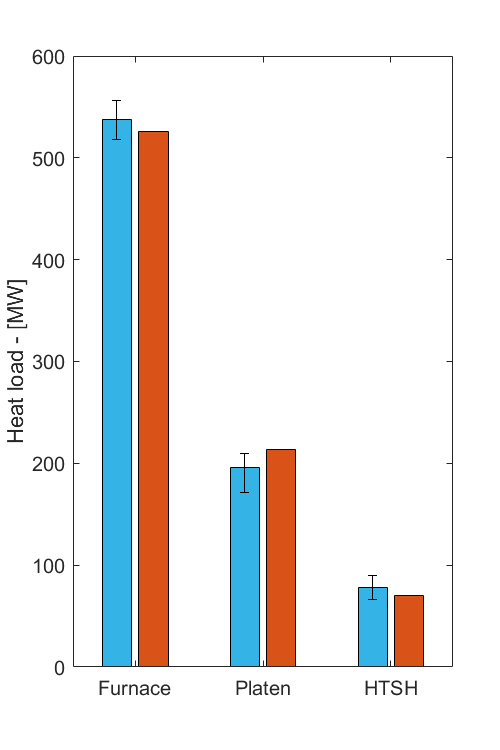
\includegraphics[width=0.32\textwidth]{100_VALID_BAR}}
	\subfigure[]{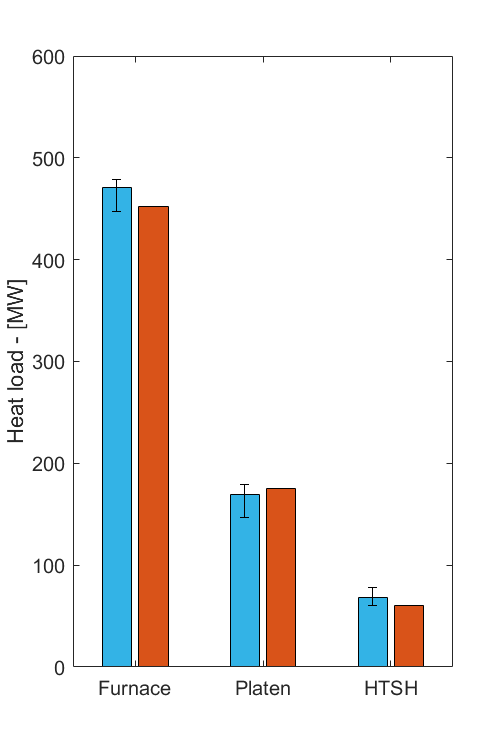
\includegraphics[width=0.32\textwidth]{80_VALID_BAR}}
	\subfigure[]{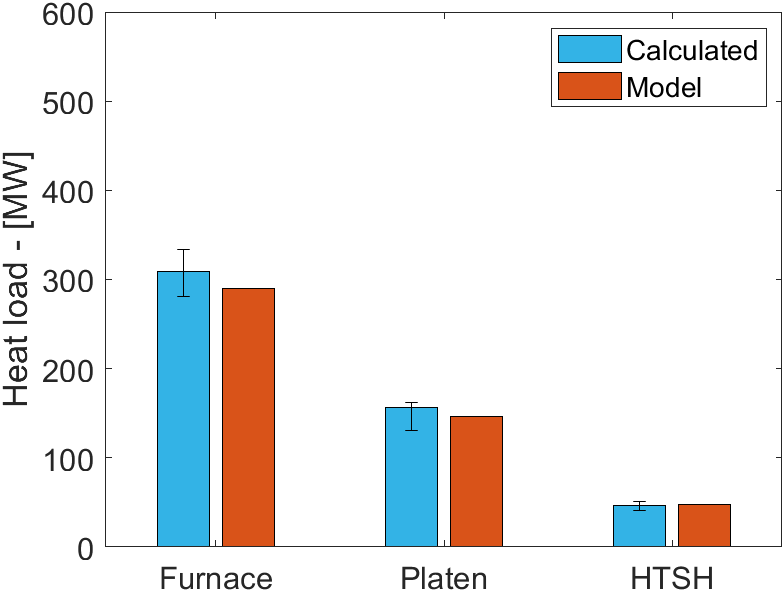
\includegraphics[width=0.32\textwidth]{60_VALID_BAR}}
\caption{Comparison of experimentally calculated and model heat loads for the furnace, platen SH and pendant SH at (a) 100\% MCR, (b) 80\% MCR and (c) 60\% MCR}
\end{figure}

In figure \ref{fig_heat_valid} it is shown that the overall heat loads are in good agreement with the measured results. For the simulated validation loads the proposed model results are within the associated error band, the general trend is an under prediction on the furnace heat loads and an over prediction on the platen super-heater. The pendant super heater illustrate the best comparable results for all load cases.\\

The CFD model was further validated by comparing the $CO_{ppm}$ and $X_{O_{2}}$ measurements against the CFD results. The probe measurements were taken at a furnace height of 37.5 [$m$] near the center of the boiler during a full load (100\% MCR) operating conditions. The probe is inserted from the side walls to a depth of 4.5 [$m$], measurements were taken every 0.5 [$m$] increment.\\
\begin{figure}[h!]\label{fig_probe_valid}
\centering
\subfigure[]{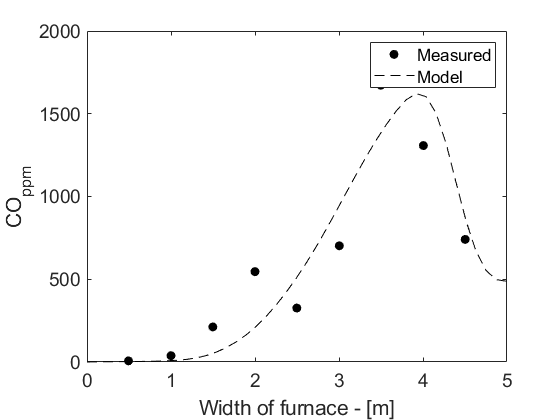
\includegraphics[width = 0.45\textwidth, height =4cm ]{COPPM_VALID}}
\hspace{5mm}
\subfigure[]{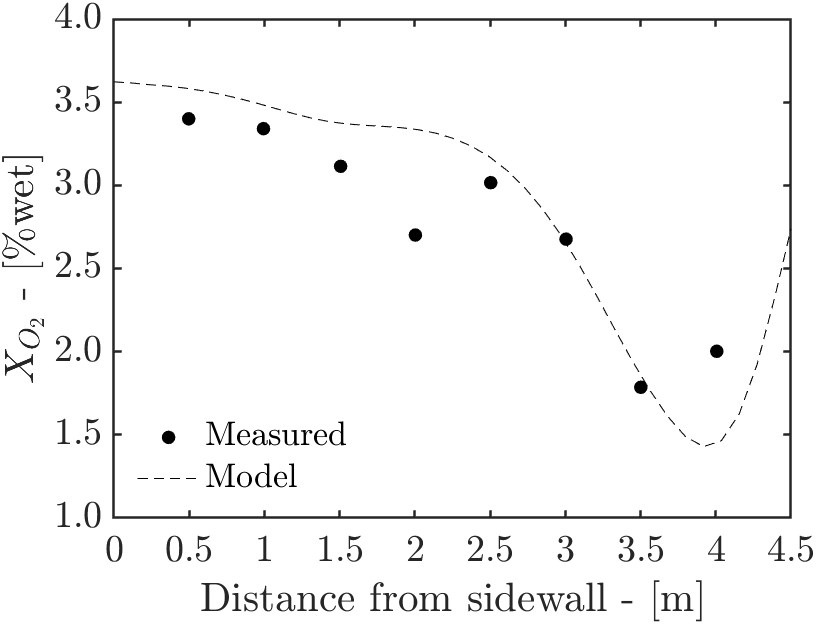
\includegraphics[width = 0.45\textwidth, height =4cm ]{XO2_VALID}}
\caption{Experimentally calculated $CO$ and $O_2$ concentration predictions}
\end{figure}

Figure \ref{fig_probe_valid} shows the averaged measurement values to that of the CFD predictions. It can be seen that the CFD model can sufficiently resolve the $CO_{ppm}$ and $X_{O_{2}}$ concentrations at the given probe location. For further information regarding the validation of the model the interested reader is directed to the works of Rawlins et al [REFERENCE]

\subsection{Simulation results for various burner firing arrangements at 32\% MCR }


Explain the investigation
table with case descriptions
Need flownex model and process modelling description
\begin{figure}
\centering
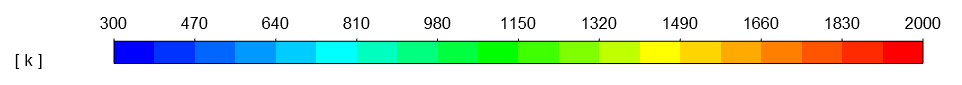
\includegraphics[scale = 0.5]{TEMP_KEY} [K]\\
\subfigure[]{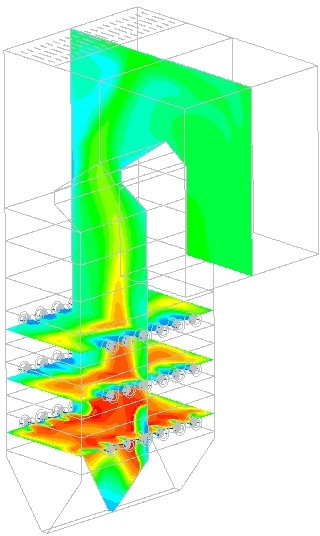
\includegraphics[width=0.32\textwidth]{BOT_TEMP}}
\subfigure[]{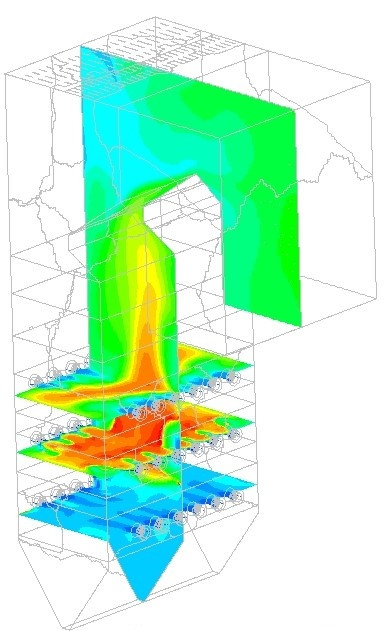
\includegraphics[width=0.32\textwidth]{MID_TEMP}}
\subfigure[]{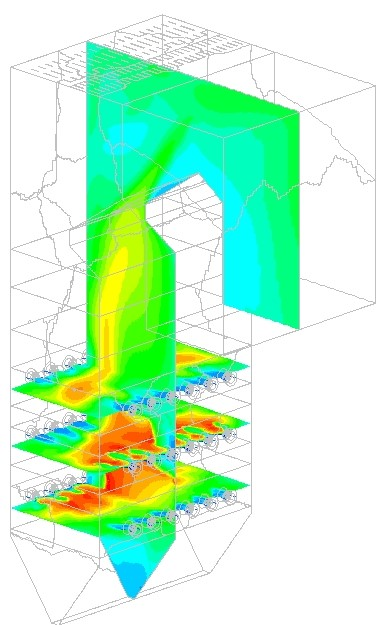
\includegraphics[width=0.32\textwidth]{FBRM_TEMP}}\\
\subfigure[]{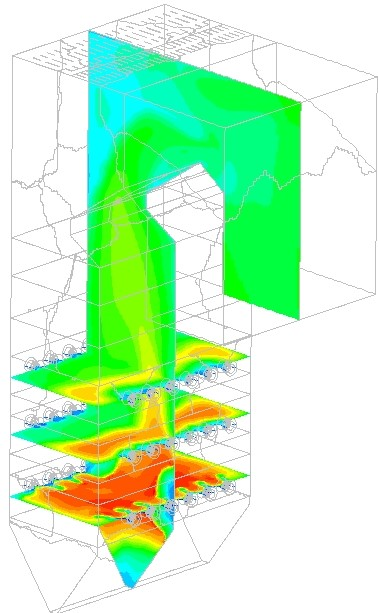
\includegraphics[width=0.32\textwidth]{BOT05_TEMP}}
\subfigure[]{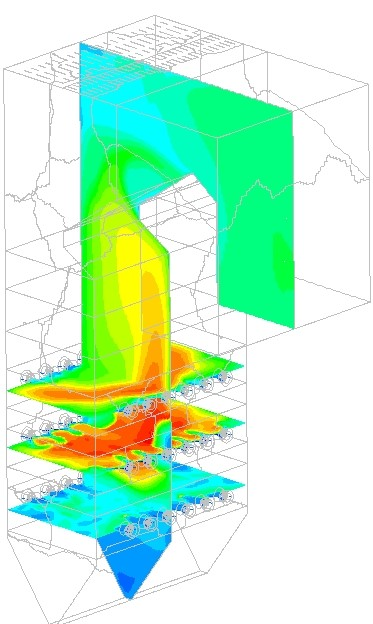
\includegraphics[width=0.32\textwidth]{MID05_TEMP}}
\subfigure[]{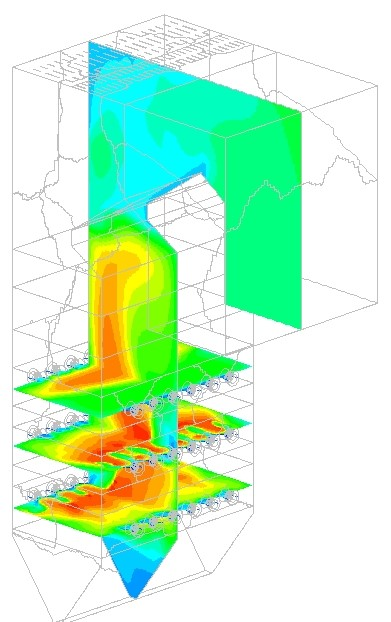
\includegraphics[width=0.32\textwidth]{FBRM05_TEMP}}
\caption{Hi}
\end{figure}


\begin{figure}[h!]
\centering
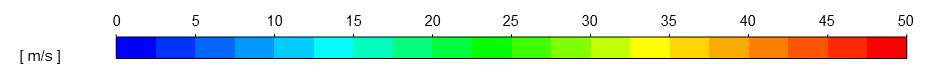
\includegraphics[scale = 0.5]{VEL_KEY}\\
\subfigure[]{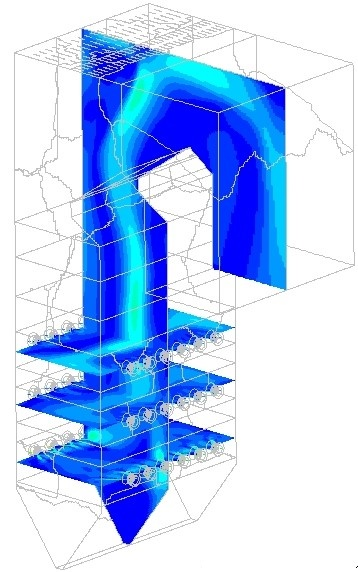
\includegraphics[width=0.32\textwidth]{BOT_VEL}}
\subfigure[]{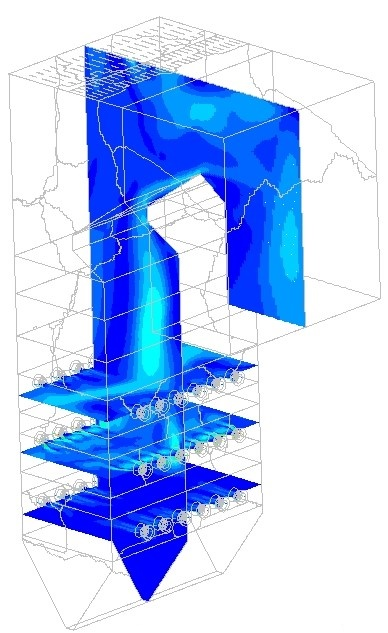
\includegraphics[width=0.32\textwidth]{MID_VEL}}
\subfigure[]{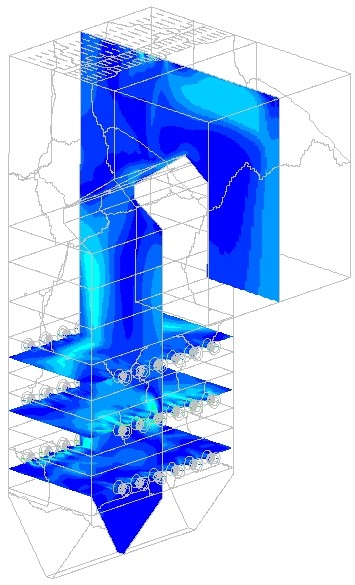
\includegraphics[width=0.32\textwidth]{FBRM_VEL}}\\
\subfigure[]{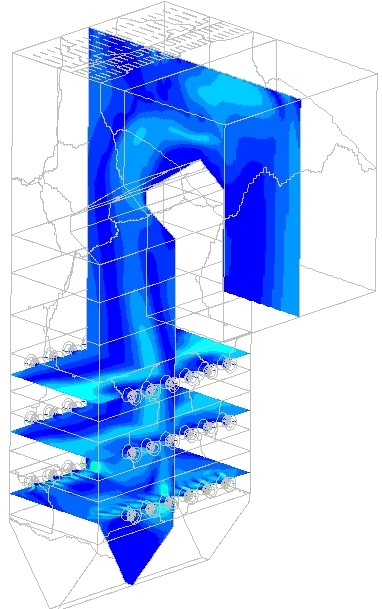
\includegraphics[width=0.32\textwidth]{BOT05_VEL}}
\subfigure[]{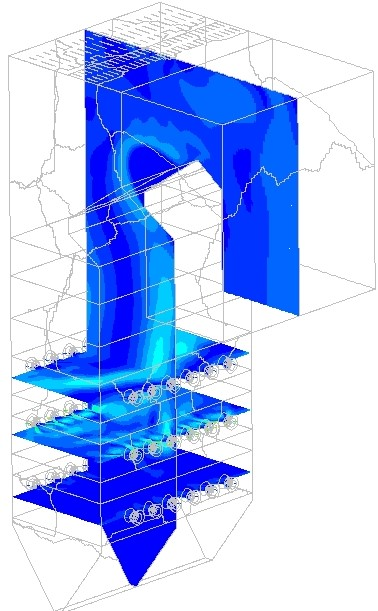
\includegraphics[width=0.32\textwidth]{MID05_VEL}}
\subfigure[]{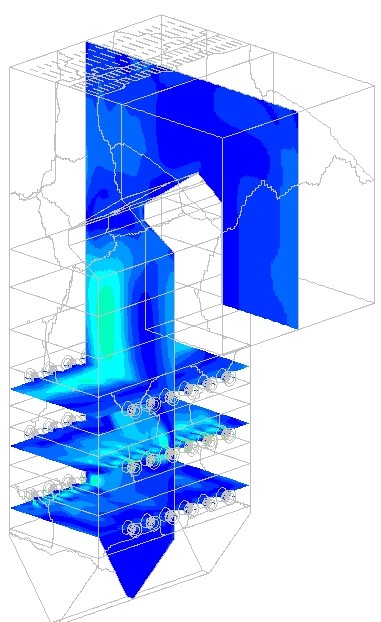
\includegraphics[width=0.32\textwidth]{FBRM05_VEL}}
\caption{bye}
\end{figure}

\begin{figure}[h!]
\centering
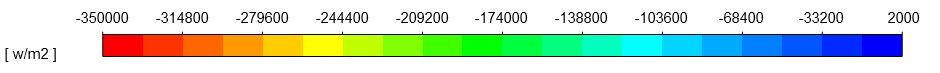
\includegraphics[scale = 0.5]{HEATFLUX_KEY}\\
\subfigure[]{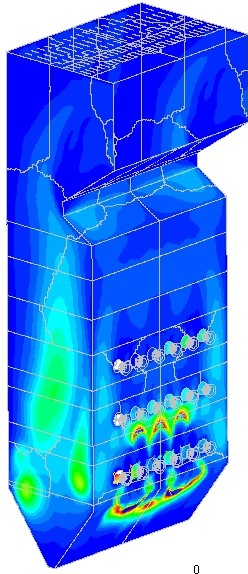
\includegraphics[width=0.32\textwidth]{BOT_HEATFLUX}}
\subfigure[]{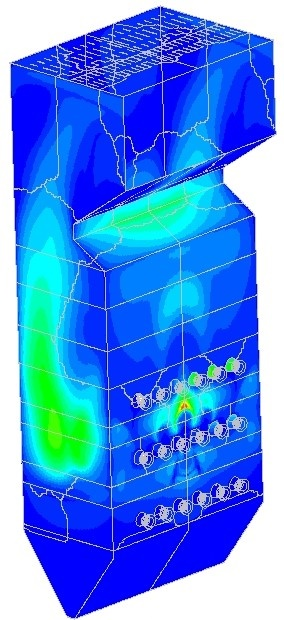
\includegraphics[width=0.32\textwidth]{MID_HEATFLUX}}
\subfigure[]{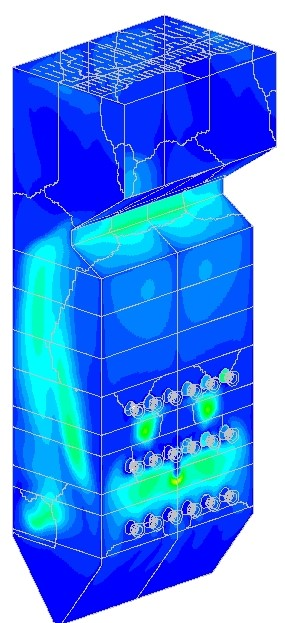
\includegraphics[width=0.32\textwidth]{FBRM_HEATFLUX}}\\
\subfigure[]{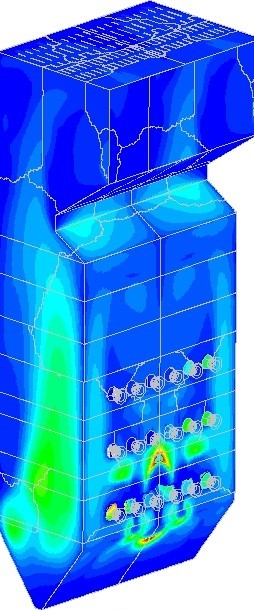
\includegraphics[width=0.32\textwidth]{BOT05_HEATFLUX}}
\subfigure[]{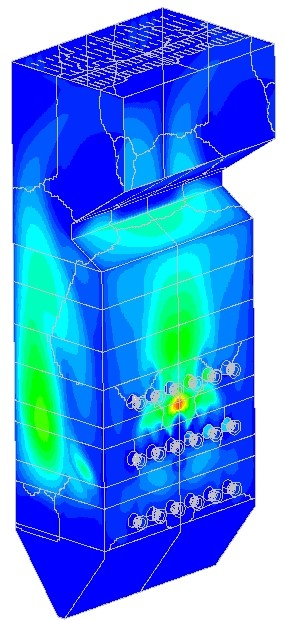
\includegraphics[width=0.32\textwidth]{MID05_HEATFLUX}}
\subfigure[]{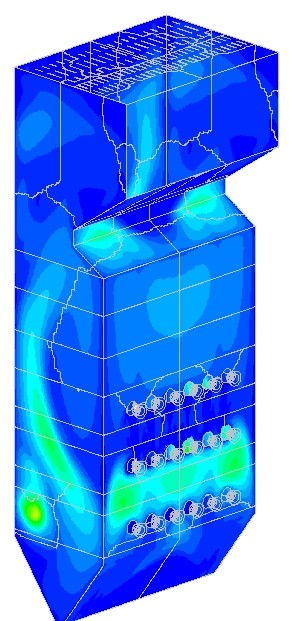
\includegraphics[width=0.32\textwidth]{FBRM05_HEATFLUX}}
\caption{bye}
\end{figure}

\begin{figure}
\centering
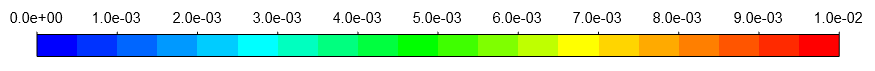
\includegraphics[scale=0.55]{CO_MF_KEY}
\subfigure[]{	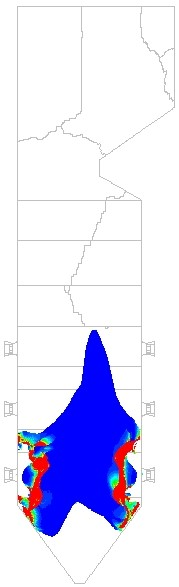
\includegraphics[width=0.18\textwidth, height = 7cm]{BOT_ISO_COPPM_F}
				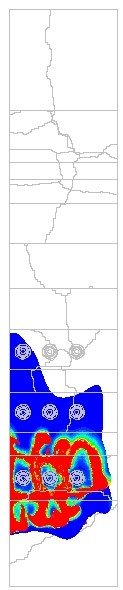
\includegraphics[height = 7cm]{BOT_ISO_COPPM_S}}
\subfigure[]{	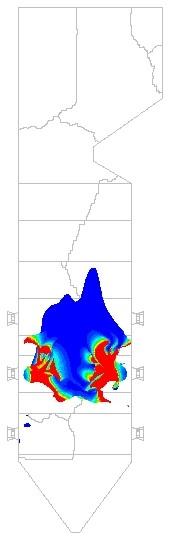
\includegraphics[width=0.18\textwidth, height = 7cm]{MID_ISO_COPPM_F}
				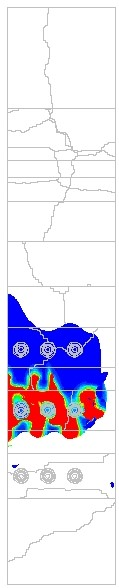
\includegraphics[height = 7cm]{MID_ISO_COPPM_S}}
\subfigure[]{	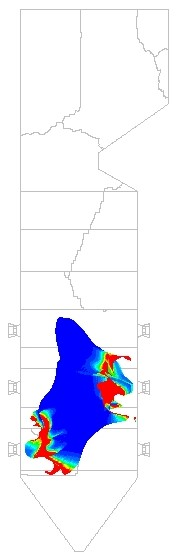
\includegraphics[width=0.18\textwidth, height = 7cm]{FBRM_ISO_COPPM_F}
				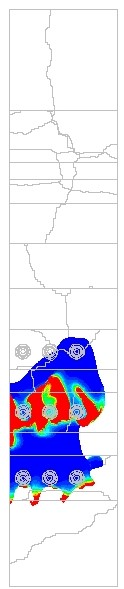
\includegraphics[height = 7cm]{FBRM_ISO_COPPM_S}}\\
\subfigure[]{	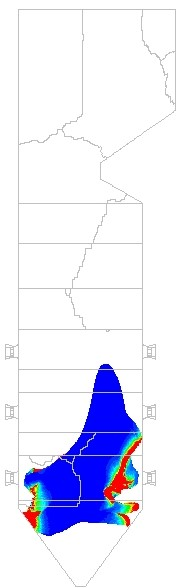
\includegraphics[width=0.18\textwidth, height = 7cm]{BOT05_ISO_COPPM_F}
				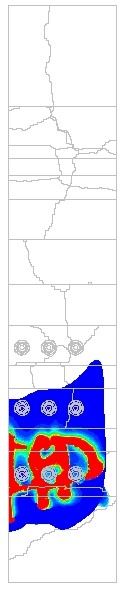
\includegraphics[height = 7cm]{BOT05_ISO_COPPM_S}}
\subfigure[]{	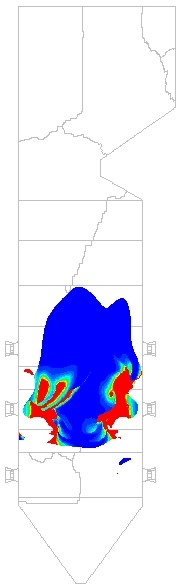
\includegraphics[width=0.18\textwidth, height = 7cm]{MID05_ISO_COPPM_F}
				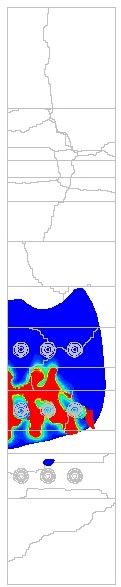
\includegraphics[height = 7cm]{MID05_ISO_COPPM_S}}
\subfigure[]{	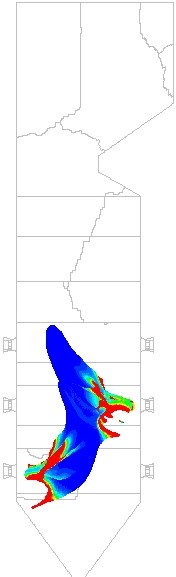
\includegraphics[width=0.18\textwidth, height = 7cm]{FBRM05_ISO_COPPM_F}
				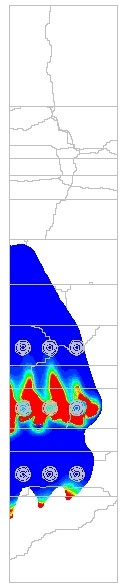
\includegraphics[height = 7cm]{FBRM05_ISO_COPPM_S}}\\
\end{figure}

\begin{table}[h!]
\centering
\caption{Utility boiler fuel characteristics}
\vspace{5mm}
\label{fuel}
{\tabulinesep=1.2mm
\begin{tabularx}{\textwidth}{l l l l l l l}
\hline
\textbf{Value} & \textbf{Case 1} & \textbf{Case 2} & \textbf{Case 3}& \textbf{Case 4}&\textbf{Case 5}&\textbf{Case 6}\\
\hline
\textbf{Platen max temp}\\
\textbf{Pendant max temp}\\
\textbf{Main steam flow rate}\\
\hline

\end{tabularx}}
\end{table}


\clearpage


\section{Conclusions}

\section{Bibliography styles}

There are various bibliography styles available. You can select the style of your choice in the preamble of this document. These styles are Elsevier styles based on standard styles like Harvard and Vancouver. Please use Bib\TeX\ to generate your bibliography and include DOIs whenever available.

Here are two sample references: \cite{Feynman1963118,Dirac1953888}.

\section*{References}

\bibliography{mybibfile}

\end{document}